\section{Location and illumination at full wave scale}\label{sec:exp}
\subsection{The inspection question and the comparison}
We use a two-metre square in air at 400 MHz. Its side is 2.67 free-space wavelengths. A pixel in the 32 and the 96 discretizations has side 62.5 and 20.8 mm, respectively. A separate seven-wave inspection of each spatial target spans 135 degrees of incidence. Nine observation angles span 146.25 degrees. There is no access to the opposite arc. The task is to locate a dielectric part from a set of possible outlines, within known tolerances on contrast and in an imperfectly known background. Outside the indicated material the background can vary independently in every pixel, from zero to $b=1/32$. The interior of a hole has this same uncertainty. A companion measurement uses the same inclusion with vacuum outside. We compute the field with the full nonlinear operator throughout. At 32 points per side the norm of the difference between the Born and full-wave data, divided by the full-wave norm, ranges from 176 to 361 percent. For the two native targets the range is 214--304 percent.

Sixteen independently generated specimens at the first resolution comprise four each of a disk, an annulus, a pair of inclusions, and an annulus with satellites. The poses and internal texture vary within each family. Two additional native-grid specimens have a ring centred at pixel $(29,66)$ and a pair centred at $(94,33)$, indexed from zero. The second pair extends past the right boundary. All positions, including edge-clipped positions, are tested. A position denotes the anchor of the specified shape, so excluding it makes no assertion that the material at that single pixel is vacuum. We use the entire noisy complex matrix and a common Frobenius error radius. A point in a retained cell of the map can have either an explicitly realized material or an unresolved existence test.

The beams used to examine two alternative amplitude patterns form a separate population. The two alternatives share a strong dielectric body and differ on two weakly uncertain lobes. They have the same permitted active region. There are 16 incident elementary waves and 16 receivers on a 168.75-degree aperture. The first illumination is available to every design, leaving 15 directions. The candidate-centre transfer contrast determines a useful empirical control; only the full intervals and old measurements enter the bounds on all materials. We distinguish a development group, enriched for a future gap near the noise, from a confirmation group selected using old data alone. The latter contains 12 independent 32-grid specimens and two independent 96-grid specimens. All policies on a specimen receive the same energy and the same absolute receiver error allowance. Apertures, noise draws, transmitted beams, and repeat exposures are paired conditions on these objects.

\subsection{What the old measurements locate}
Table~\ref{tab:cover} gives whole-field results for a specified shape. A verified material was found at every generating centre in the primary tests. For the sixteen 32-grid specimens, the largest cover contained twelve cells and the smallest one. Using all four possible outlines together, all 48 alternatives with incorrect shape were excluded at every centre. For the correct outline, the centre cover and its witness were unchanged. Scanning a single full-wave material template at the midpoint of the specified inclusion interval with vacuum outside ranked the generating centre first on all sixteen smaller specimens and on the native annulus. On the clipped native pair it ranked the generating centre second, one cell away from its preferred position. Even the best nominal point residuals were 3.61--6.81 noise radii on the smaller grid and 4.54--5.29 on the native grid. We therefore fitted a common core amplitude and homogeneous background on the five best nominal centres of every specimen. The selected positions recovered all eighteen centres, including the clipped pair. The fitted residuals at the two native centres were $1.0043r$ and $1.0094r$ (in ascending order); only one of eighteen fitted media passed full-wave error verification. This fit used 3,151 full-wave point evaluations, with 68.69 seconds for fitting and 0.52 seconds for independent readback on the same machine, in addition to the original template sweep. Allowing spatially varying material then yielded a witness at all eighteen centres. These comparisons give no point-location advantage to the set method. They distinguish a correct centre from a physically admissible dielectric and from a bound on all alternative locations. An orthogonality-sampling backpropagation indicator placed its largest value at the generating centre on three specimens and placed it within its five highest pixels on five. This indicator ranks pixels by a physical correlation. Without an independent outer error bound on the rank it provides a different output from a set containing all possible centres.

\begin{table}[tb]\centering
\caption{Possible inclusion centres before a further exposure at 3 percent noise. The discrete model and the stated outline and contrast intervals are assumed here. An exclusion applies to every material in that class. The witness column counts centres with a checked material. Unresolved centres are retained. Alternative specifications on the same specimens are paired conditions.}\label{tab:cover}
\small\begin{tabular}{@{}lrrrr@{}}\toprule
Material class and grid & Tested & Excluded & Witness & Unresolved\\\midrule
Specified layer, sixteen $32^2$ & 16384 & 16313 & 16 & 55\\
Specified layer, $96^2$ annulus & 9216 & 9099 & 1 & 116\\
Specified layer, $96^2$ clipped pair & 9216 & 9192 & 1 & 23\\
Uncertain layer, four $32^2$ annuli & 4096 & 2381 & 4 & 1711\\
Uncertain layer, $96^2$ annulus & 9216 & 8243 & 1 & 972\\\bottomrule
\end{tabular}\end{table}

To isolate the effect of an uncertain background we evaluated the receiver-direction perturbation bound at the same centres. With the exterior known to be vacuum it excluded 16,301 of 16,384 centres, compared with 16,349 using the combined tests. Allowing each exterior cell up to $1/32$ left the perturbation test without a single exclusion. The inverse of the centre-field propagator still exists, but the absolute majorant for scattering by the exterior is too large. The material sector treats exterior power jointly before taking a receiver norm. This difference is substantial even for a weak background; it does not establish failure of every possible perturbation inequality.

Widening the material tolerance reveals the role of the negative current space. The primary inspection specifies a half-amplitude boundary layer around each core. In the wider inspection the core cells vary independently in $[3,5]$ and the boundary cells independently in $[0,5]$. The four 32-grid annuli then give 555, 568, 616 and 642 excluded centres. The successful state matrices have two to five negative directions. On the native annulus, all 8,243 strict exclusions in this wider class use an indefinite state. Relaxing the boundary description makes the potential positions more numerous even with unchanged readings.

A zero count from a finite positive-weight search need not indicate a physical obstruction. We therefore compare with continuously variable nonnegative weights on the background and the footprint. At one tested annular position the continuous search found a positive state whose verified distance lower bound exceeded the receiver radius by $0.5927$. At one different position of each of the four 32-grid annuli we exhibited a nonzero current in the exact receiver null space. Both its footprint-sector and background-sector energies were strictly negative on the original operator. Any nonzero nonnegative combination has a negative direction at that position, for every positive overall scale and every positive semidefinite receiver weight. The indefinite test excludes all four positions. This identifies both an actual obstruction and an example where a better positive search succeeds. Independently varying optical weights at every pixel constitute a larger comparison class.

\begin{figure}[tb]\centering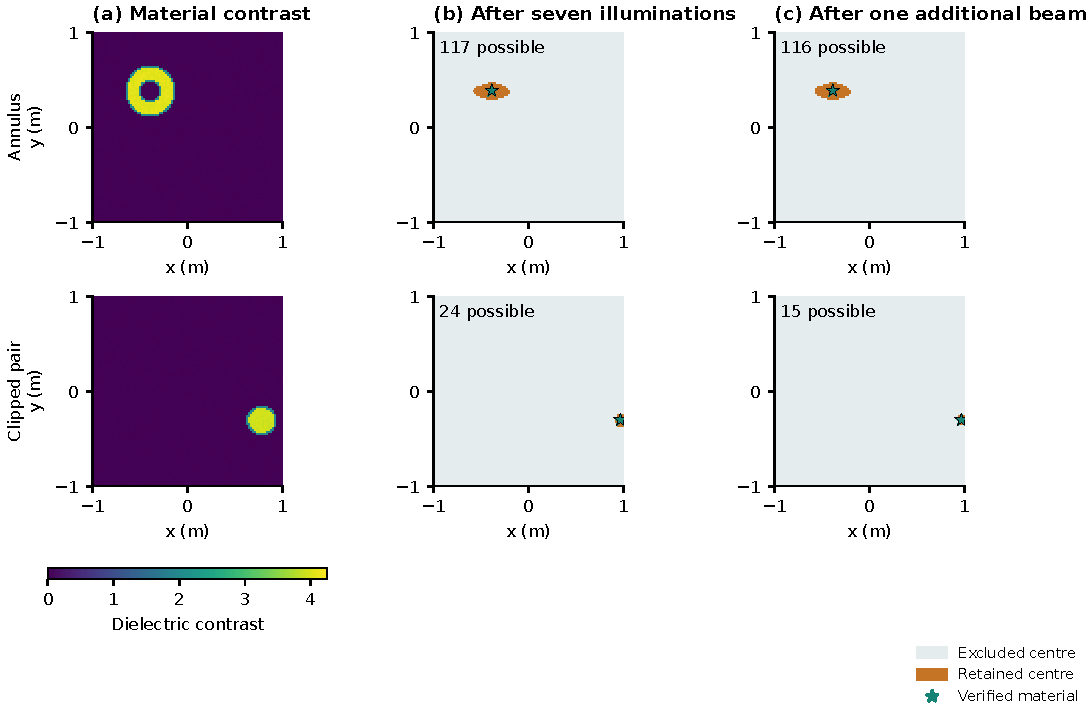
\includegraphics[width=\linewidth]{location}
\caption{Whole-field tests on the two 96 by 96 specimens. The first column gives the generating material for scoring. The central column uses seven old illuminations. Orange cells retain a possible centre and the star denotes a centre with a verified material. The final column uses one further coherent illumination. In the clipped pair the admissible region lies against the outer boundary. All three panels in a row have the same spatial extent.}\label{fig:loc}
\end{figure}
\begin{figure}[tb]\centering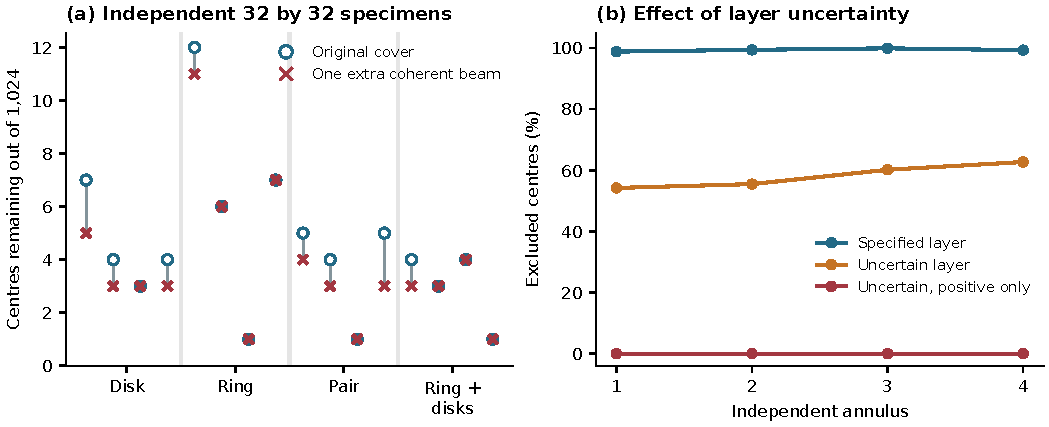
\includegraphics[width=\linewidth]{population}
\caption{Location cover and material tolerances. Left, each pair of marks belongs to one independent specimen with uncertain exterior. Right, the reduction in excluded centres when boundary contrast is released. The positive-state curve uses the same finite menu restricted to positive states. The continuous-weight comparison in the text addresses the limitation of this control.}\label{fig:population}
\end{figure}

A position test also permits a conditional amplitude question. We retain the shape and pose and replace the amplitude specification by adjacent intervals. At the native annulus the interval $[2,3]$ and the interval $[3,3.75]$ for the core profile are inconsistent, while a material in $[3.75,4.25]$ fits the data. A box constraining every core value to the same interval asks a different question from bounding an arbitrary isolated pixel. For example, failure of the low box means at least one value exceeds its upper endpoint, conditional on the other geometric and material constraints. A separate independent-cell peak-cap test at the returned centre gives a strict lower bound of 3.0 for the native annulus and 2.5 for the clipped pair. The upper bound remains at the imposed maximum of 6.0. Each has a witness with peak 4.25. The detector cannot assign the largest value to an individual pixel. A more permissive task must also test mixtures that straddle the bin boundaries.

The noise sensitivity in Figure~\ref{fig:phase} uses one predetermined specimen of each 32-grid shape and both native specimens. New complex noise draws share the physical targets. On the first grid we re-evaluate all the centres. On the native grid we transfer the strict 3 percent distance lower bound $d_3$ using the 1-Lipschitz dependence of a distance on the observed field: $d(y')\geq d_3-\|y'-y_3\|_F$. This conservative alternative avoids recomputing clipped edge geometries. At 10 percent in the unknown background the two native counts are 8,903 and 9,177 strict exclusions. At 1 percent the original native witnesses failed the tighter transfer check. Refitting them on the noisy readings gave verified residuals below 0.863 and 0.753 of the new radius for the two weak-background specimens. Physical witnesses were found on both grids for all 36 paired background and noise conditions. The noise figure counts physical centres across paired targets, including any unresolved cells.
\begin{figure}[tb]\centering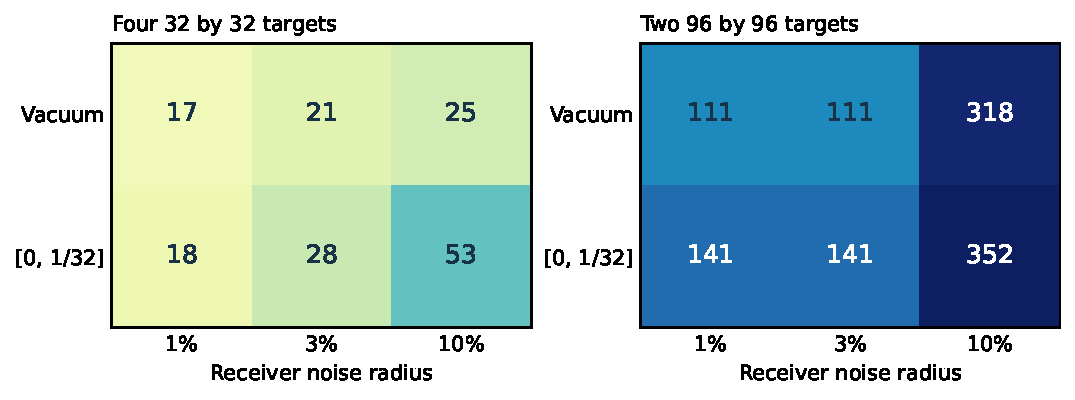
\includegraphics[width=.93\linewidth]{noise_phase}
\caption{Numbers of centres retained over the whole field as background uncertainty and receiver noise change. Each row represents data generated in the indicated background, and inversion uses the matching background contract. The denominators are 4,096 on the left and 18,432 on the right. Full recomputation on the left and a transferred native bound on the right have different sensitivity to lowering the noise.}\label{fig:phase}
\end{figure}

\paragraph{How much a change of discretization costs.}
To test the effect of resolution, we also average each of the two native materials over $3$ by $3$ blocks and solve a new 32-grid volume integral equation with the same physical sources and receivers. Coincident incident fields agree to $9\times10^{-16}$ relatively. Receiver rows are expressed in the native angular quadrature units. Relative to the clean 96-grid measurements the differences are 15.82 percent for the annulus and 6.77 percent for the clipped pair. They amount to 5.27 and 2.26 times the stipulated receiver error. Against the actual noisy readings the coarse solutions give residuals of 5.28 and 2.44 noise radii. Adding these sample discrepancies to the original radius would require factors 6.28 and 3.26 after rounding upwards. These are measured discrepancies for two materials. A model-error bound covering the whole material class would be required to transfer an exclusion between grids.

\subsection{Costs of an indefinite position or amplitude update}
To measure the cost of changing a box we use two arrays for which the common parent gives an unresolved answer. One has 1,024 state coordinates and seven negative directions. The second has 9,216 electromagnetic cells and 1,153 possible current cells with nine negative directions; the remaining cells are exactly vacuum in this timing experiment. Width and midpoint changes at three locations give a rank-four signed update. There are 1,000 distinct, nonnested changes on each specimen, of which 757 and 472 are excluded, respectively. Counts from the reduced matrices agree with direct original-state computations for all the changes. Four predetermined changes on each grid undergo a separate original-operator interval evaluation. An exactly singular control with a null current coupled to a source exercises the retained border in \eqref{eq:augment}.

Two full-wave amplitude controls put the widths in context. A low-contrast disk (peak $0.625$) and a hollow ring (peak $3.50$, first-Born field error $376\%$) occupy the same permitted 1,153-cell circular region, with different actual supports. Against the same solid tapered specification centred at peak four, the excluded widths are approximately $5.14$ and $3.09$ times the Neumann norm cutoff, respectively. In each case a permitted perturbation has spectral radius above one (lower bounds $1.086$ and $1.389$). These fixed-position controls are separate from the whole-field location cohort.

For the first grid the first hundred original factorizations took 52.4 seconds and the thousand took 870.6 seconds. Once the common matrices were prepared the corresponding 128-bit reduced runs took 0.090 and 0.955 seconds. Including common input, setup and all thousand reduced checks costs 96.7 seconds. Adding the four independent original-state interval checks increases the cost to 382 seconds. The measured original-state and reduced floating-point CPU times for the thousand changes are 582.9 and 0.117 seconds. For the second grid a thousand direct numerical factorizations took 1,157 seconds and the prepared interval updates took 5.56 seconds. With all preprocessing and four original-operator checks included the cost was 342 seconds. At just a hundred tests the fully charged reduced runs were slower on both grids: 234 versus 52 seconds and 238 versus 83 seconds, respectively. The amortization becomes visible only after enough changes have been tested. These paired timings concern equal inertia decisions at the same threshold. They do not compare the time to a reconstructed image. On both grids an admissible upper-endpoint perturbation had spectral radius strictly above one, with respective lower endpoints 1.0010 and 1.1083. A centre-series contraction in any induced norm therefore fails for that perturbation.

A fresh multiscale comparison used four predetermined 32-grid specimens and both native spatial specimens with uncertain background. A strict parent test removed 1,740 of 4,096 centres before individual testing on the first grid and 9,359 of 18,432 on the second. All 3,361 successful parent tests had a negative state direction. For the native annulus alone, 366 groups of nine centres were excluded in one test per group. Evaluating the remaining leaves anew gave exactly the same complete cover as an independent scan of every leaf, on every specimen. All six full-wave witnesses survived. The individual centre--weight evaluations fell from 4,208 to 2,468 and from 18,714 to 9,355, respectively. With identical shared state preparation, the measured online times for grouped versus flat evaluation were 8.45 versus 3.71 seconds over the four smaller targets and 78.92 versus 29.04 seconds over the two native targets. Within the native multiscale run, 51.07 seconds were spent factoring the parent classes. With the common state and clipping preparation charged, the totals were 247.57 versus 197.69 seconds. Forming the wider spatial classes costs more than the saved leaf tests on these arrays. For this application we use direct translated tests when online latency is the objective.

A whole-field position scan has a different setup cost. The native annulus has 625 distinct clipped edge geometries. Computing location-independent state information for the primary native annulus took 317 seconds; the subsequent port calculations for the two background measurements took 62 seconds together. Reusing an interior plan for the wider annulus required 103 seconds for the original interior calculation and a further 282 seconds for the full field. Charging both prevents the inexpensive repeats of one fixed local change from standing in for the cost of a new geometry.

\subsection{The value of a further illuminated field}
For location alone the three already unique 32-grid covers need no further exposure. On the other thirteen, an additional uniform direction left all 68 old possible centres. A random angle left 66, the best individually selectable angle left 57 and coherent illumination left 58. The last two designs used nominal responses of representatives in the old cover; every previously retained centre was tested after the acquisition. All four policies retained every generating centre. For all sixty follow-up observations a full-wave material at the returned centre fits the two separate error balls. The original material sufficed in 49 measurements; a bounded refit at the same centre sufficed in the remaining eleven. The maximum verified residuals were 0.988 and 0.979 of the old and new radii, respectively. The native clipped pair changed from 24 possible centres to 18 under uniform incidence and to 15 for either optimized choice. For the annulus its 117 possible centres changed to 116 under uniform incidence, 115 with the best single angle and 116 with the coherent wave. A favourable beam for discrimination of two classes need not be favourable for many adjacent positions.

We next ask a question for which a guaranteed improvement in the reading has operational significance. Can a single acquisition distinguish two surviving material specifications for \emph{all} admissible new errors? At a preliminary common fluence of $0.014$ old-shot units, a verified physical pair in each of the fourteen confirmation cases had full-dictionary maximum difference below $2r_a$. Changing the beam alone could not meet that demand. We then used only the old data and a stored pair of indefinite conditional forms to set the energy for a target separation of $2.15r_a$. The energy is common to all competing policies within each specimen. The twelve energies at the first resolution ranged from 0.0352 to 0.491, with median 0.0778. The two native energies were 0.1778 and 0.4200. All cases had one negative state direction and one positive old-data direction per material class. The old-data-conditioned bound exceeded $2r_a$ in all fourteen, and a new measured field eliminated the wrong class in all fourteen. Forward evaluation gave a material in the surviving class each time. These counts at target-selected energies should be read together with the independent necessary-energy bounds in Figure~\ref{fig:energy}.

\begin{figure}[tb]\centering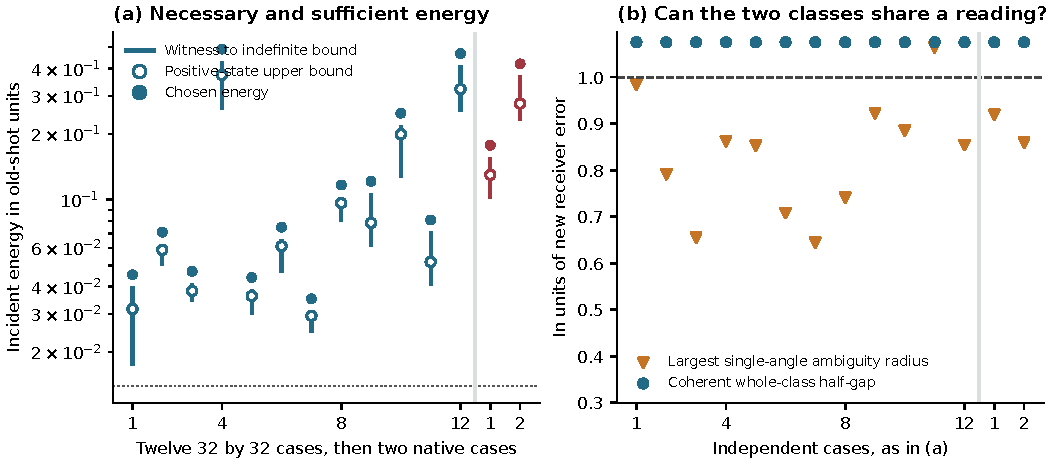
\includegraphics[width=\linewidth]{energy}
\caption{Paired incident-energy comparisons on the fourteen confirmation specimens. Left, lower endpoints use actual old-compatible materials; upper endpoints use whole classes and the indicated state. Filled dots give the energy used before recording a new field. Right, an orange value below one establishes a common reading for \emph{every} elementary angle, while a blue value above one guarantees separation under the coherent command. The vertical divider separates the grids.}\label{fig:energy}
\end{figure}

The necessary and sufficient energy brackets obtained with the indefinite forms are $[0.1034,0.1539]$ and $[0.2344,0.3636]$ for the two native specimens (endpoints rounded outwards). The lower endpoint uses two physical materials compatible with the same old reading. The positive-state calculation improves the sufficient endpoints to 0.1302 and 0.2761, rounded upwards. The classical coherent wave from the two centre transfer matrices, evaluated with the same positive form, already gives sufficient energies of 0.1335 and 0.2831. The numerical evidence supports a benefit from coherent hardware and from reasoning about material classes. It does not establish an advantage in reconstructing material over the classical eigenwave of two known transfer matrices.

With a single transmitter at a time, common readings exist on all fifteen admissible directions in eleven of the twelve 32-grid cases and in both native cases, at the very energy used by the successful coherent command. On the remaining small-grid specimen the result covered thirteen of fifteen directions. For the native specimens the largest upper bounds on the common-reading error over all angles were 0.9191 and 0.8590 times $r_a$. Equation~\eqref{eq:transcript} extends this obstruction to time sharing at fixed total incident energy and one joint receiver error budget. It is independent of which measured field happened to be drawn.

On the actual measurements, in contrast, the best Fisher angle and the centre-discrimination eigenwave both selected the correct class on all twelve 32-grid specimens and both native specimens when either of the same two verified forms could exclude a class. With the indefinite form alone the Fisher, uniform and random counts on the first grid were seven, eight and two. Uniform and random directions each succeeded on eleven of twelve and on both native specimens. This observation is consistent with the common-reading counterexamples: set separation protects against an adverse reading, whereas a particular noise draw can be easy to classify. Additional diagnostic calculations in the development group were used to adjust state weights. Their success rates are not pooled with confirmation.

Finally we asked how many elementary waves must be driven \emph{simultaneously}. On the first native specimen one transmitter is insufficient and three suffice, giving a minimum of two or three. On the second specimen the exact minimum is two. A command on the directions $67.5$ and $90$ degrees has a strictly positive gap of $0.0921r_a$ after subtracting both error radii. A receiver-direction projection of the full-wave real material secant, including its bounded higher-order remainder, sharpens the quadratic test on this borderline pair. Independent native-operator norm enclosures for the two classes of the second specimen give $\eta<0.01438$ in \eqref{eq:realwidth}. The two native three-transmitter quadratic distances are at least $2.1026r_a$ and $2.1095r_a$. In one 32-grid case all 455 triples admit a common physical reading and a four-transmitter distribution gives $2.0200r_a$, proving a minimum of four. Thus the hardware question can have a definite answer even while much of the material remains undetermined.


\begin{table}[tb]\centering
\caption{Three sparse-hardware results at the chosen incident energy. The impossibility column uses an old-compatible physical pair for every indicated subset of transmitters. The two remaining columns concern the entire material intervals. A successful realized readout alone contributes nothing to the necessary count.}\label{tab:ports}
\small\begin{tabular}{@{}llll@{}}\toprule
Specimen & Insufficient simultaneous ports & Sufficient & Minimum\\\midrule
$32^2$, case three & every triple (455/455) & 4 & 4\\
$96^2$, first & every individual (15/15) & 3 & 2--3\\
$96^2$, second & every individual (15/15) & 2 & 2\\\bottomrule
\end{tabular}
\end{table}

The full-wave witness upper bounds on two-port capability were also evaluated on all 105 pairs on each native specimen. They ruled out 100 pairs for the first and 97 for the second. With the second specimen the real-contrast receiver projection in \eqref{eq:realwidth} proved four of the eight remaining pairs sufficient. After committing these restricted commands, new full-wave readings retained a physically realized true class on both specimens and removed the false class even on the first specimen, for which two-port sufficiency is still unresolved. Computing all candidate support scores of sizes one through four and the full set, from cached quadratic forms, took 1.06 seconds for the two native cases. The physical witness bounds took a separate 4.75 seconds, and refining the two-port real-contrast receiver directions took another 4.76 seconds. Original-operator evaluation of the fourteen experiments, including competing policies and their readouts was considerably more expensive: the twelve small-grid objects took 38.3 seconds and the two native objects 132.3 seconds. These costs include the numerical verification and are separate from measurement energy.
